\clearpage

\section{\MET\ Templates from \gjets\ Sample}
\label{app:templates}

In this section we display the templates used for the inclusive analysis (red) and the targeted analysis (blue).

\begin{figure}[!h]
\begin{center}
\begin{tabular}{cc}
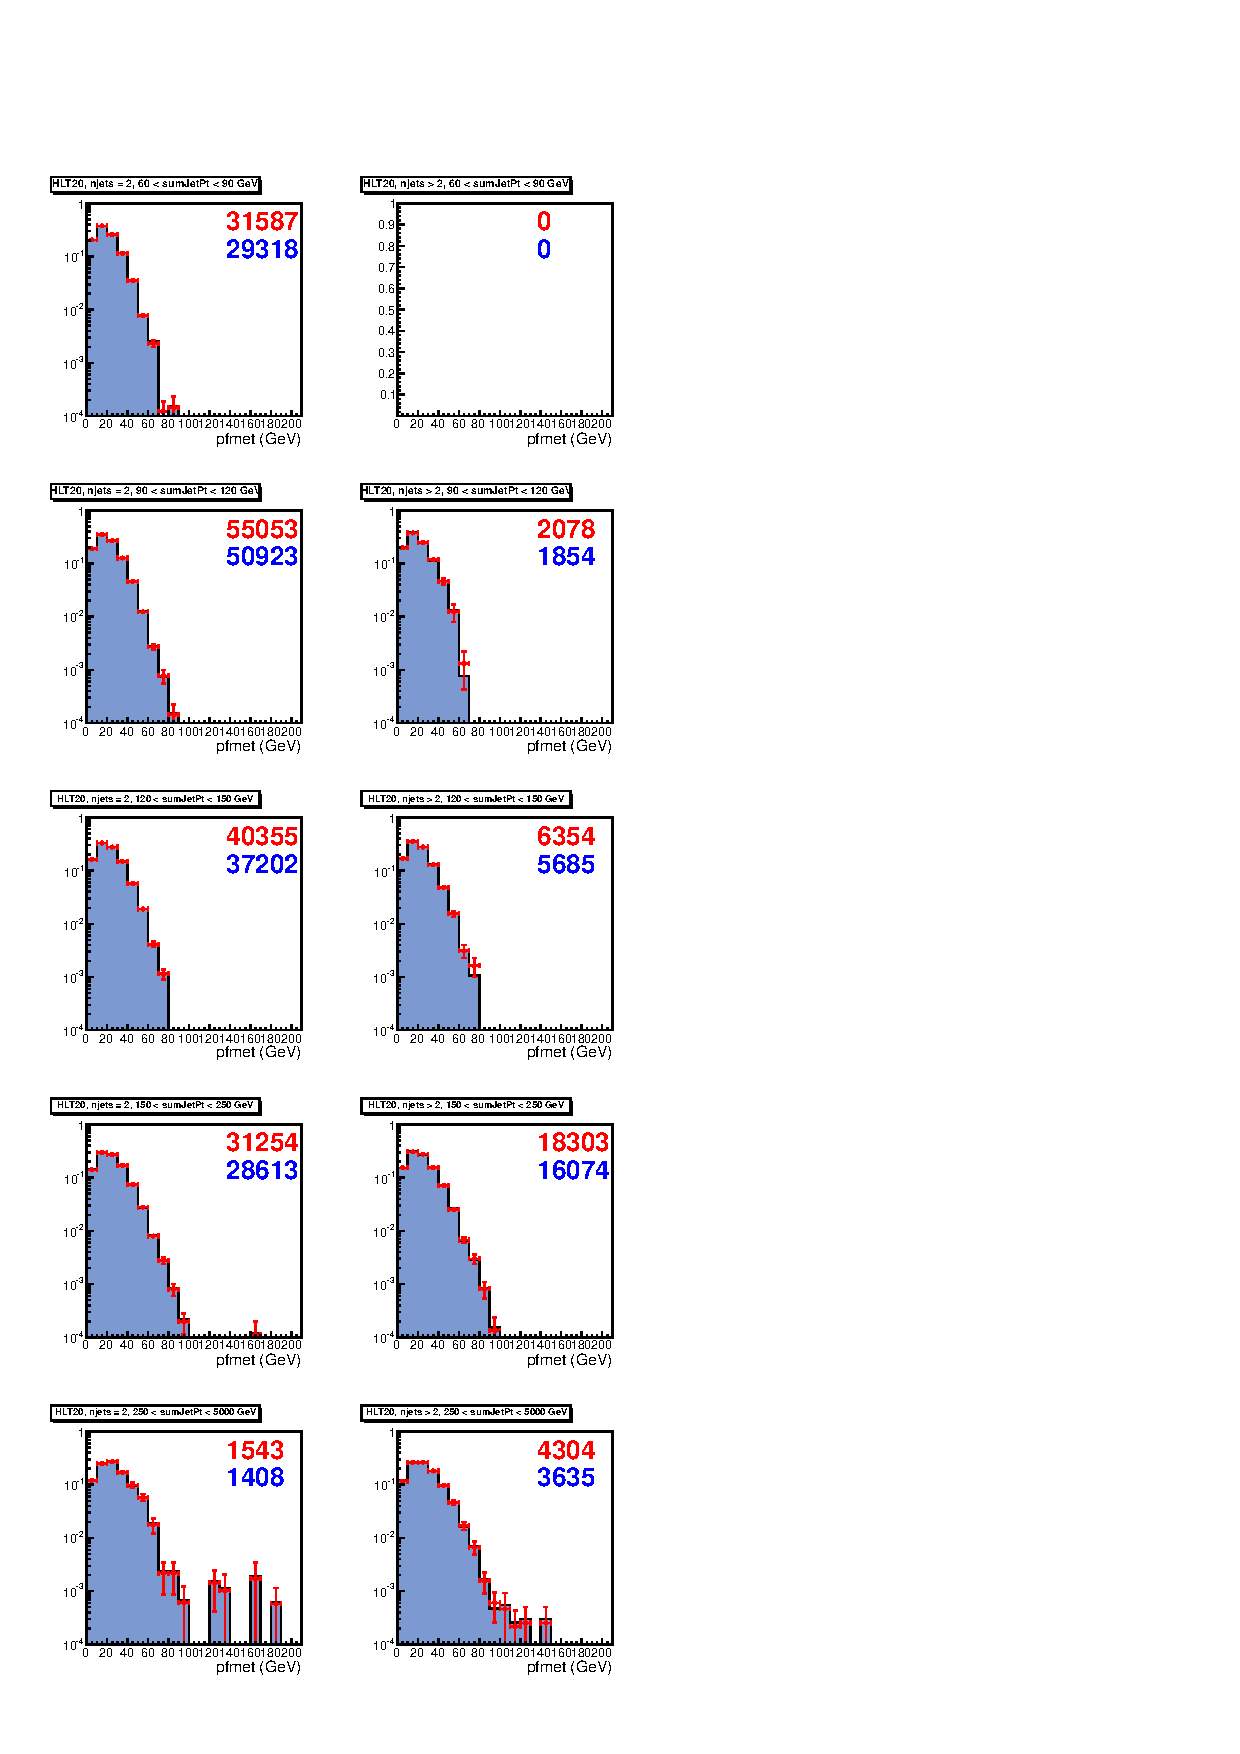
\includegraphics[width=0.5\textwidth]{plots/template_targeted_0_19fb.pdf}
\end{tabular}
\caption{
\MET\ templates collected with the \pt $>$ 22 GeV single photon trigger.
The number in red (blue) indicates the number of entries in the template for the inclusive (targeted) analysis.
}
\end{center}
\end{figure}

\clearpage

\begin{figure}[!h]
\begin{center}
\begin{tabular}{cc}
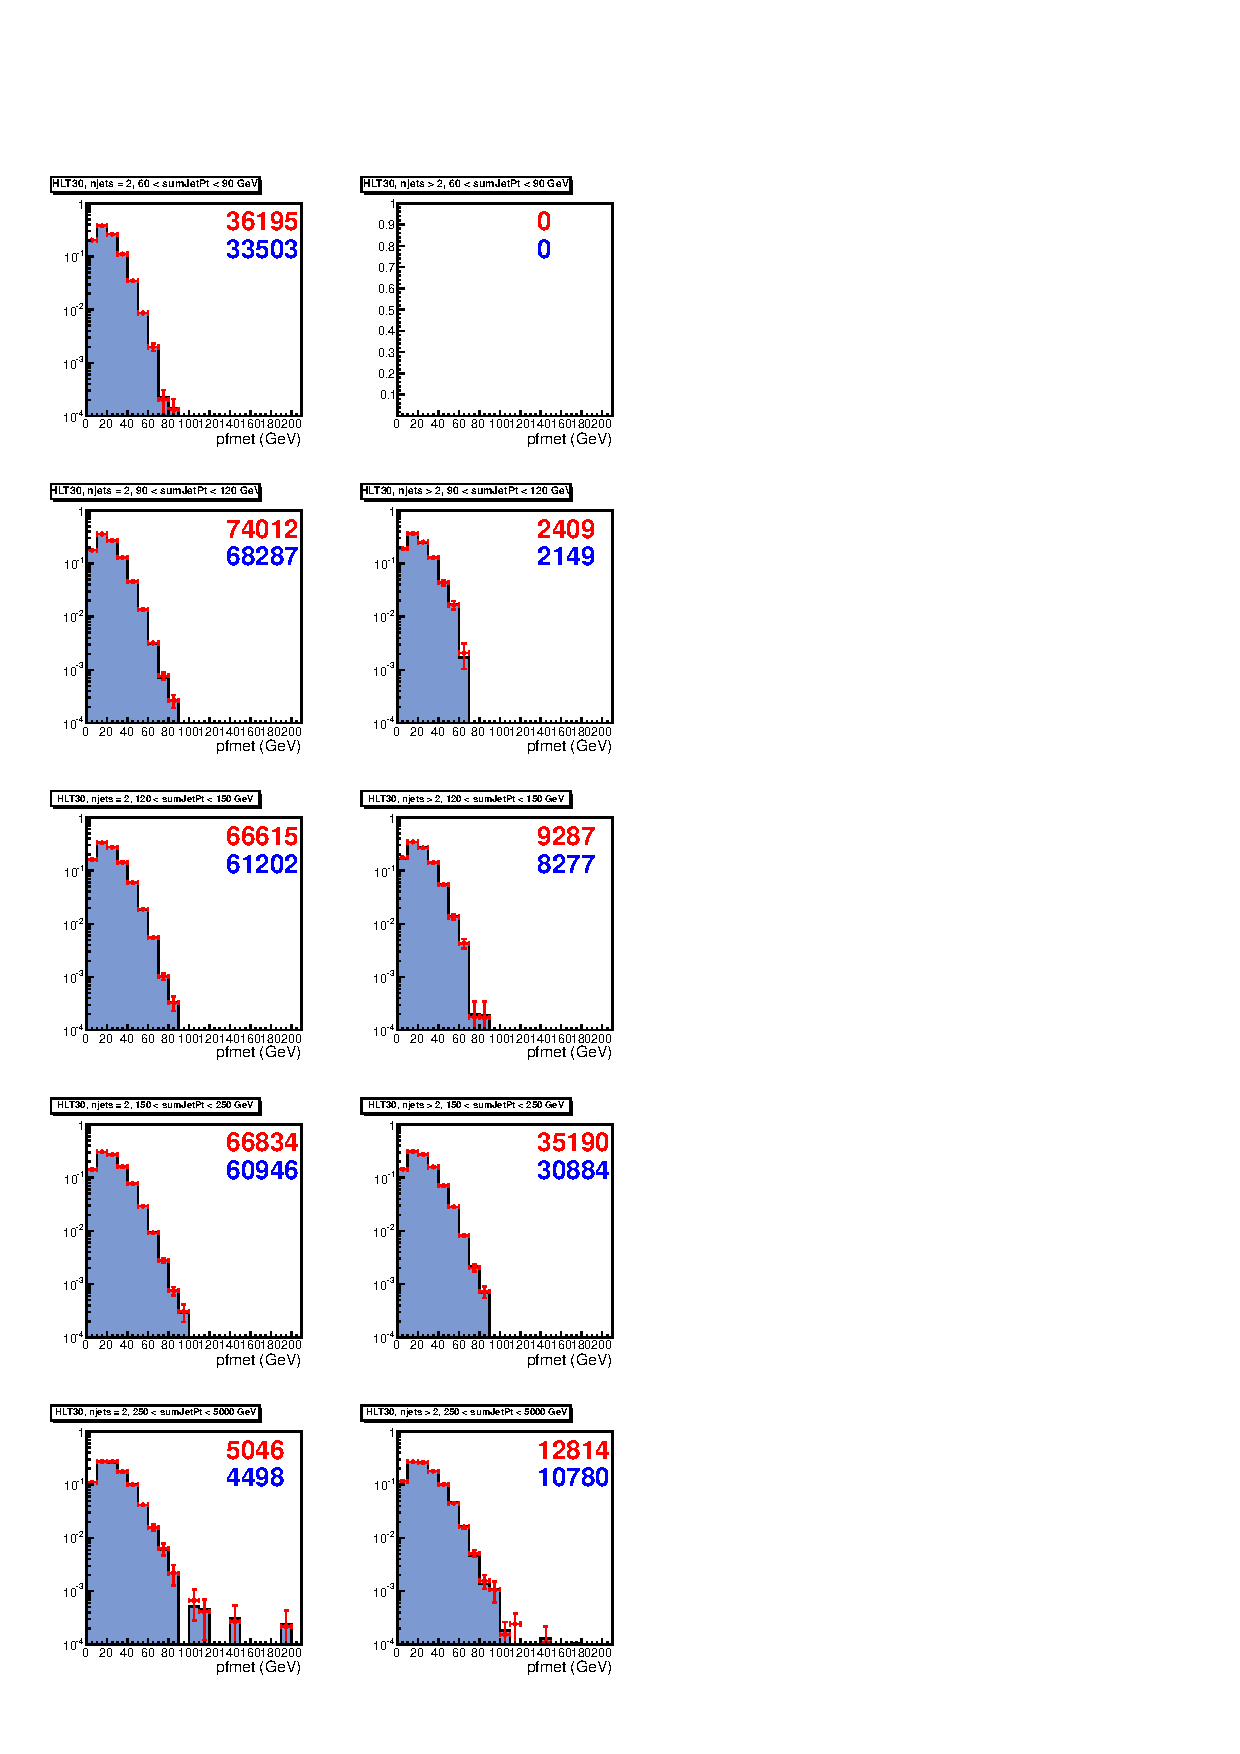
\includegraphics[width=0.5\textwidth]{plots/template_targeted_1_19fb.pdf}
\end{tabular}
\caption{
\MET\ templates collected with the \pt $>$ 36 GeV single photon trigger.
The number in red (blue) indicates the number of entries in the template for the inclusive (targeted) analysis.
}
\end{center}
\end{figure}

\clearpage

\begin{figure}[!h]
\begin{center}
\begin{tabular}{cc}
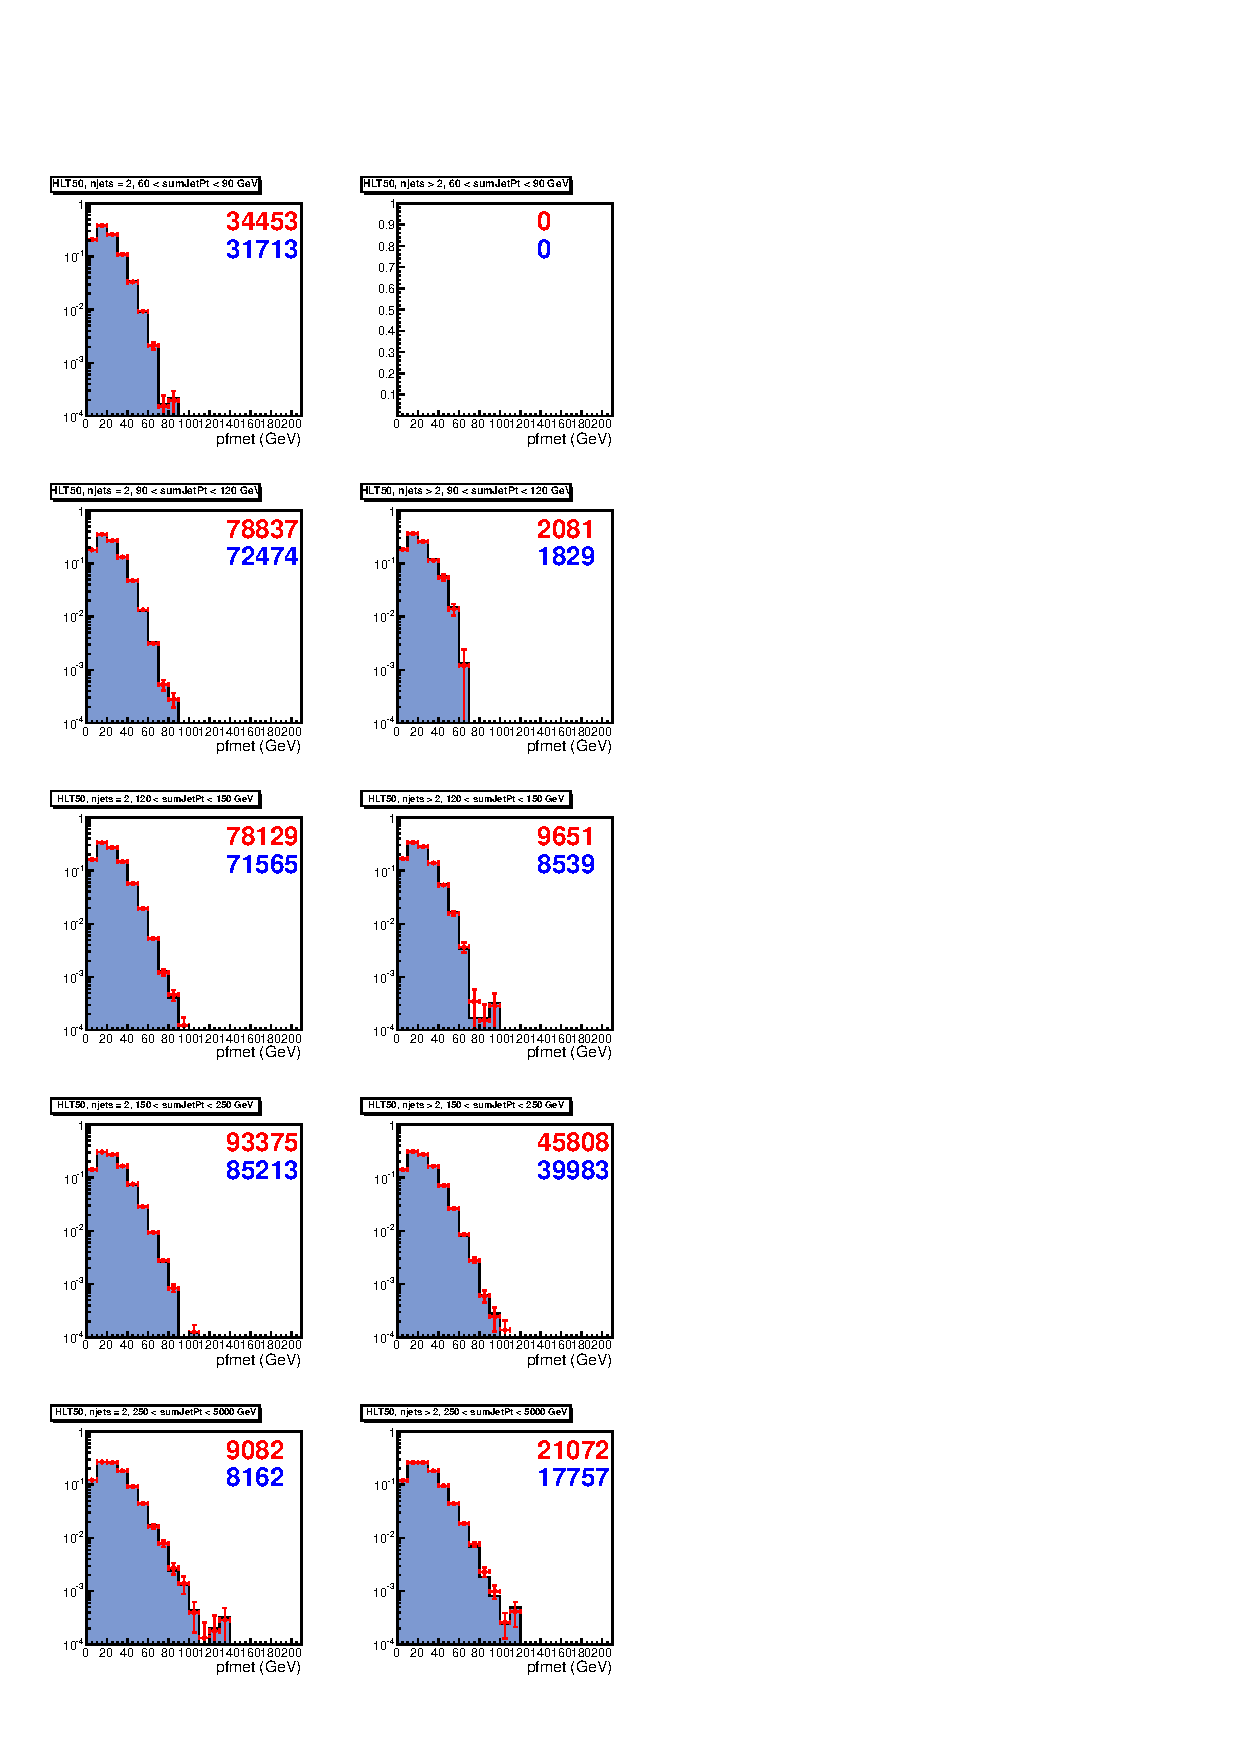
\includegraphics[width=0.5\textwidth]{plots/template_targeted_2_19fb.pdf}
\end{tabular}
\caption{
\MET\ templates collected with the \pt $>$ 50 GeV single photon trigger.
The number in red (blue) indicates the number of entries in the template for the inclusive (targeted) analysis.
}
\end{center}
\end{figure}

\clearpage

\begin{figure}[!h]
\begin{center}
\begin{tabular}{cc}
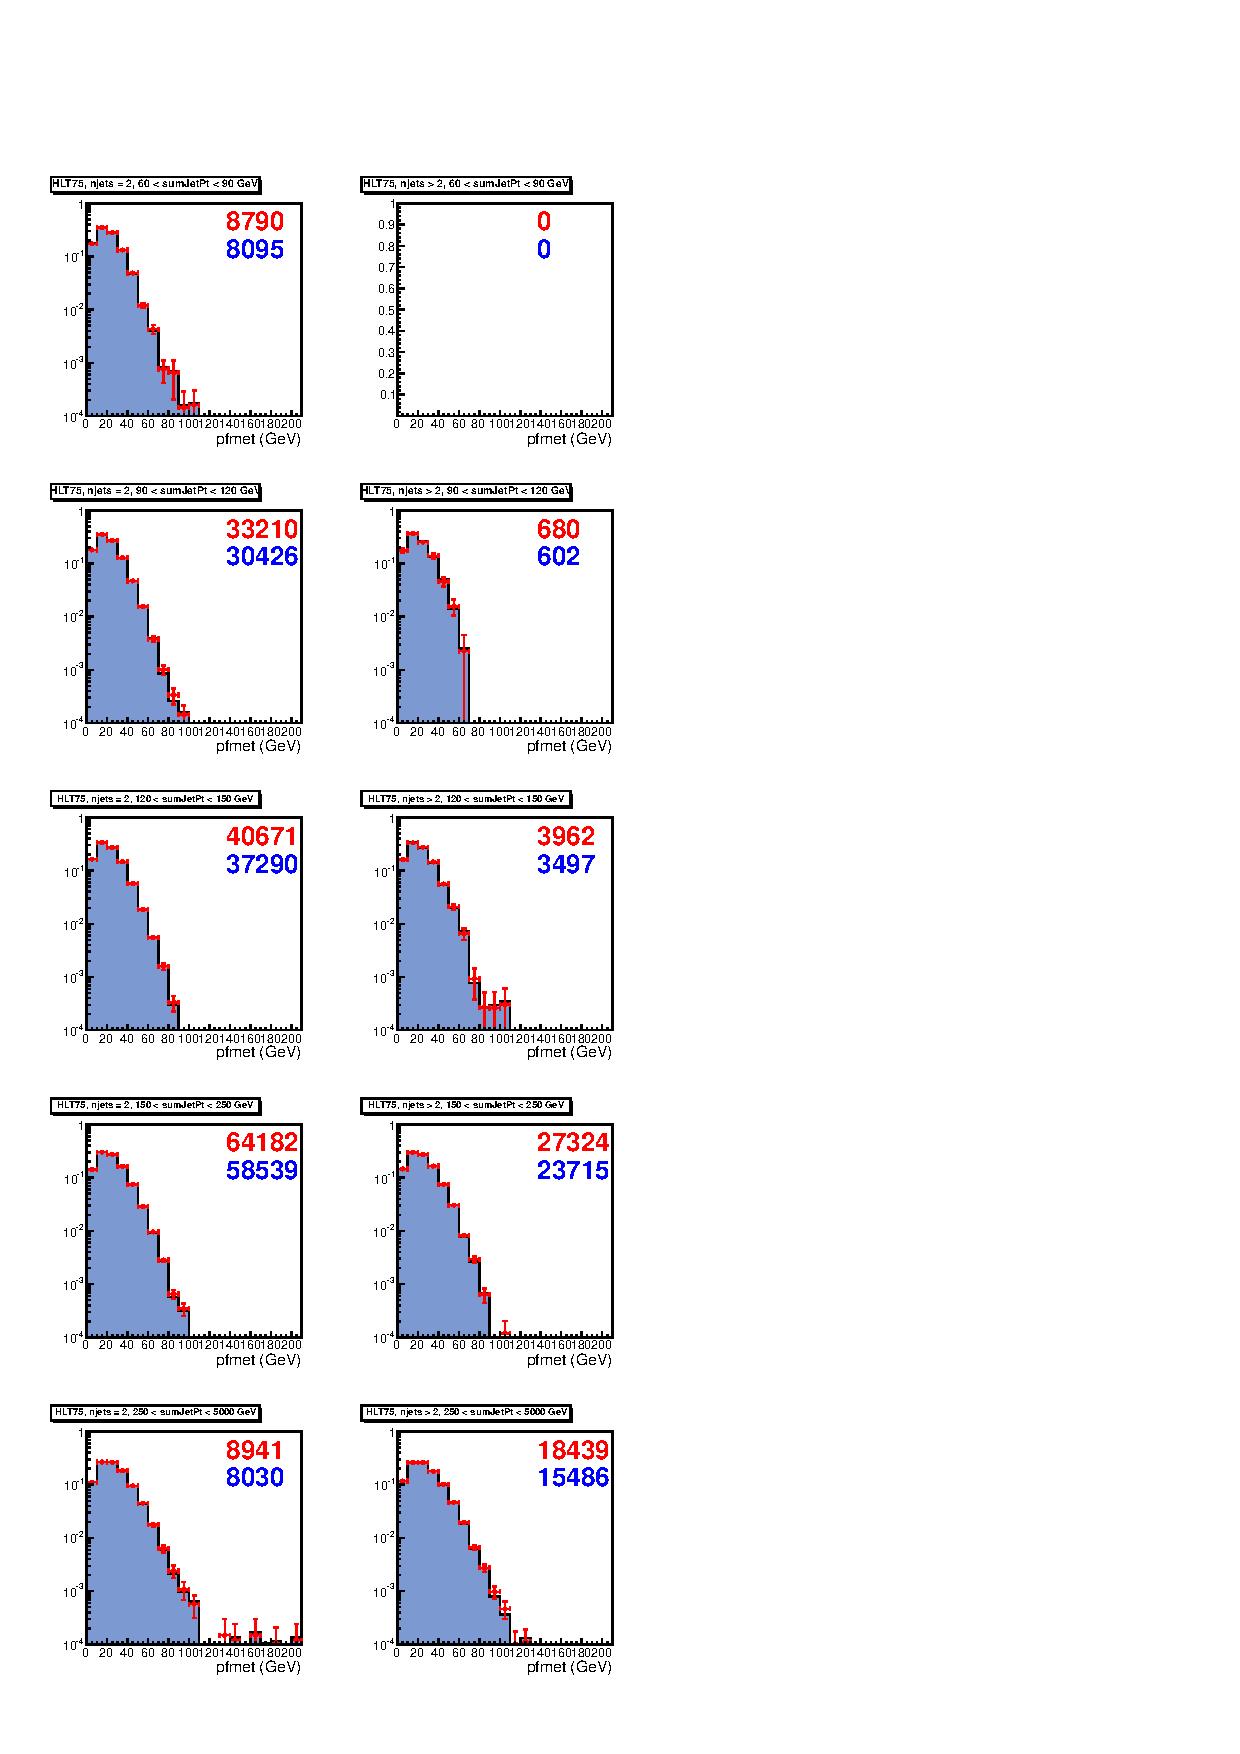
\includegraphics[width=0.5\textwidth]{plots/template_targeted_3_19fb.pdf}
\end{tabular}
\caption{
\MET\ templates collected with the \pt $>$ 75 GeV single photon trigger.
The number in red (blue) indicates the number of entries in the template for the inclusive (targeted) analysis.
}
\end{center}
\end{figure}

\clearpage

\begin{figure}[!h]
\begin{center}
\begin{tabular}{cc}
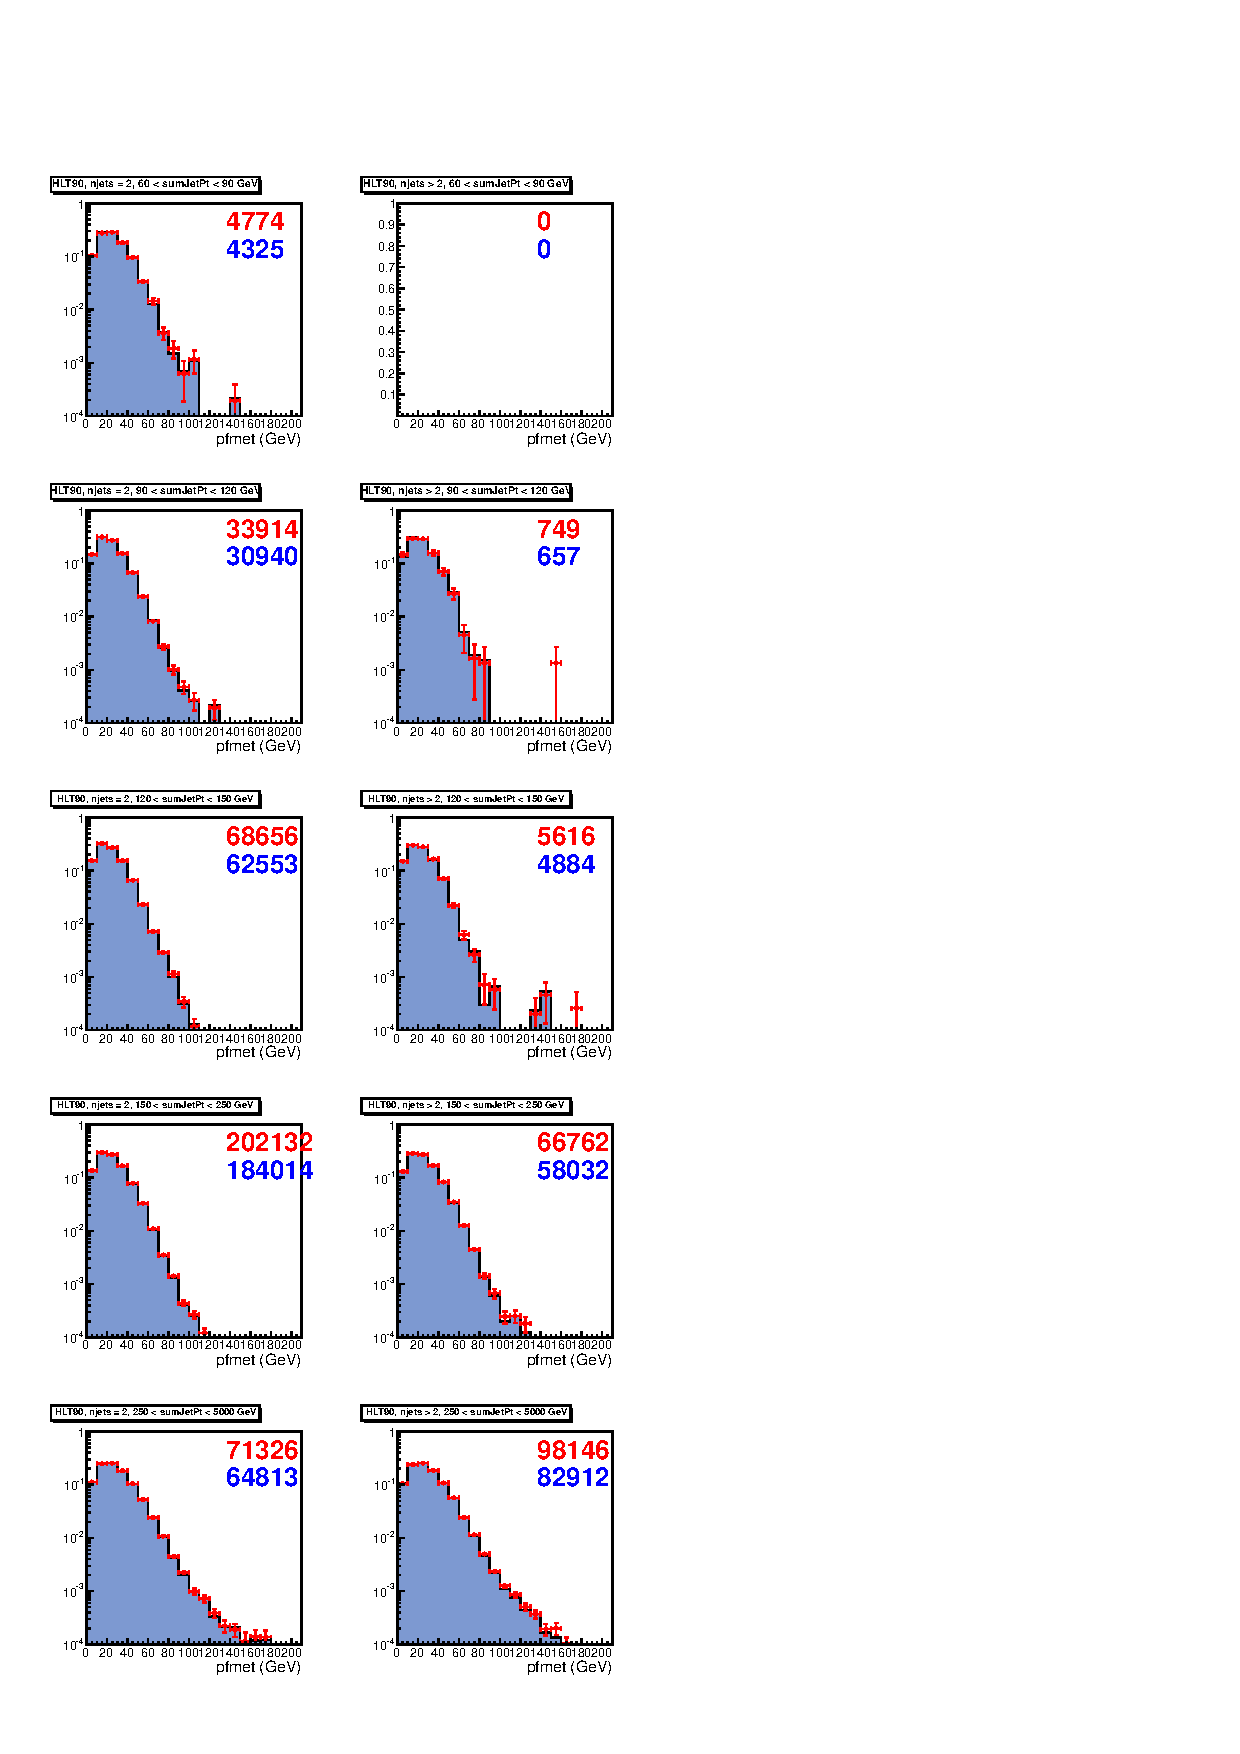
\includegraphics[width=0.5\textwidth]{plots/template_targeted_4_19fb.pdf}
\end{tabular}
\caption{
\MET\ templates collected with the \pt $>$ 90 GeV single photon trigger.
The number in red (blue) indicates the number of entries in the template for the inclusive (targeted) analysis.
}
\end{center}
\end{figure}
